\chapter{Results}
\lhead{\chaptername~\thechapter. \emph{Spherical SfM}}
In this chapter we comment the results obtained with our SfM pipeline.
We tested our approach with both some computer-generated and real environments.
We compare the pose estimation results with ground truth in the synthetic cases
while we only give a qualitative evaluation for the multi-view stereo
reconstruction step for both the syntetic and real video sequences.
We obtained all the results with MATLAB R2017a on a \todo{aggiungere caratteristiche macchina laboratorio}

\section{Synthetic Scenes}
The first synthetic environment is a simple one we created in Blender 2.78c;
it is composed of a room with 5 polyhedrons. We added some image textures to both
the room's walls and the shapes' faces to reduce matching outliers.
The camera moves in a continuos curve around the polyhedron and both its
position and orientation change.
Figure~\ref{fig:test6} shows some rendered images for this environments.
%
\begin{figure}
\centering
	\begin{subfigure}{0.4\textwidth}
		\centering
		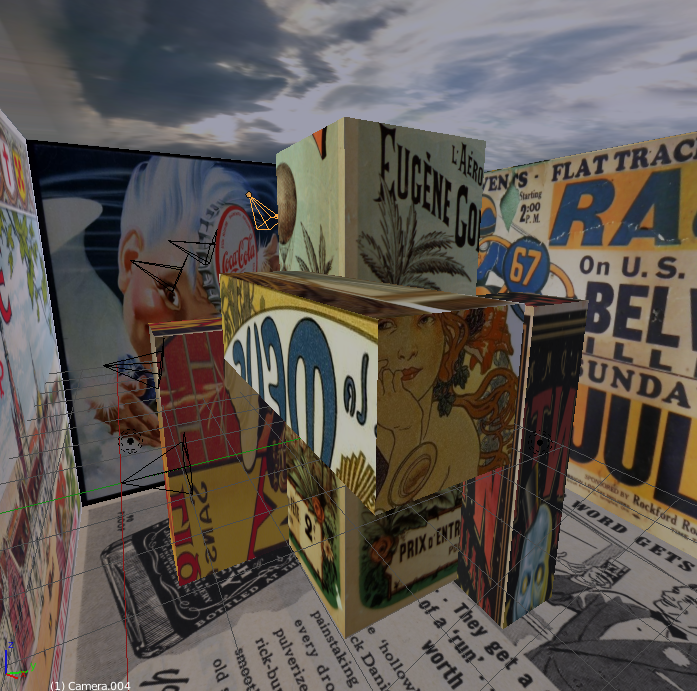
\includegraphics[width=\textwidth]{img/test6_1}
	\end{subfigure}
    %
	\begin{subfigure}{0.4\textwidth}
		\centering
		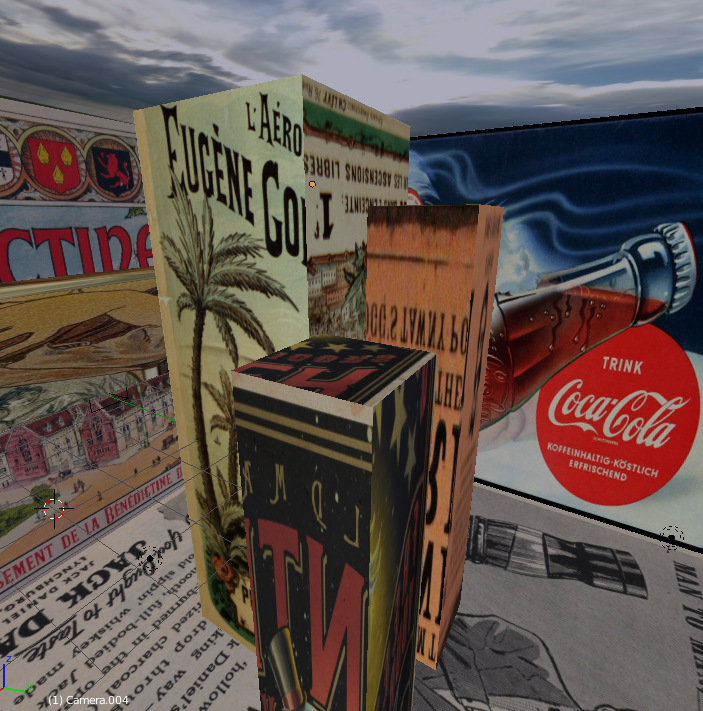
\includegraphics[width=\textwidth]{img/test6_2}
	\end{subfigure}
    %
	\begin{subfigure}{0.4\textwidth}
		\centering
		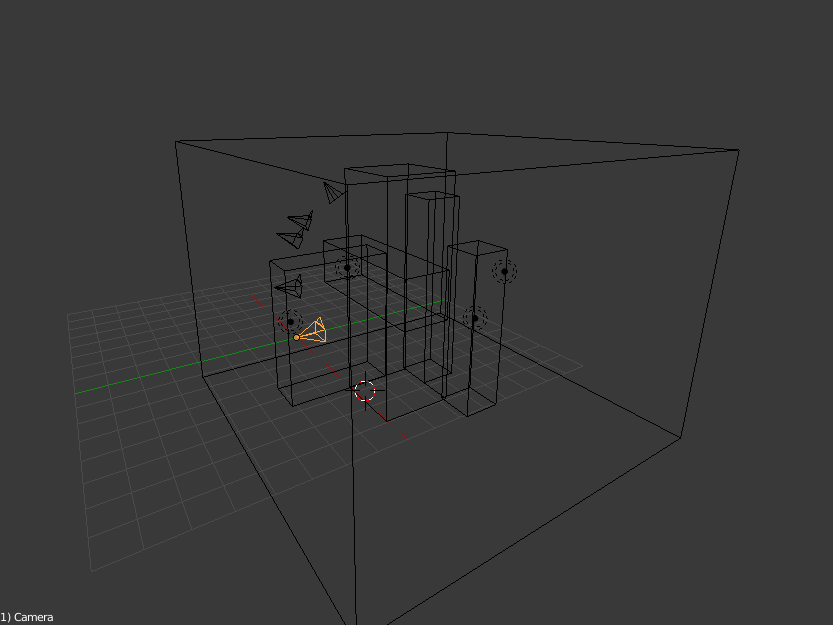
\includegraphics[width=\textwidth]{img/test6_3}
	\end{subfigure}
    %
	\begin{subfigure}{0.4\textwidth}
		\centering
		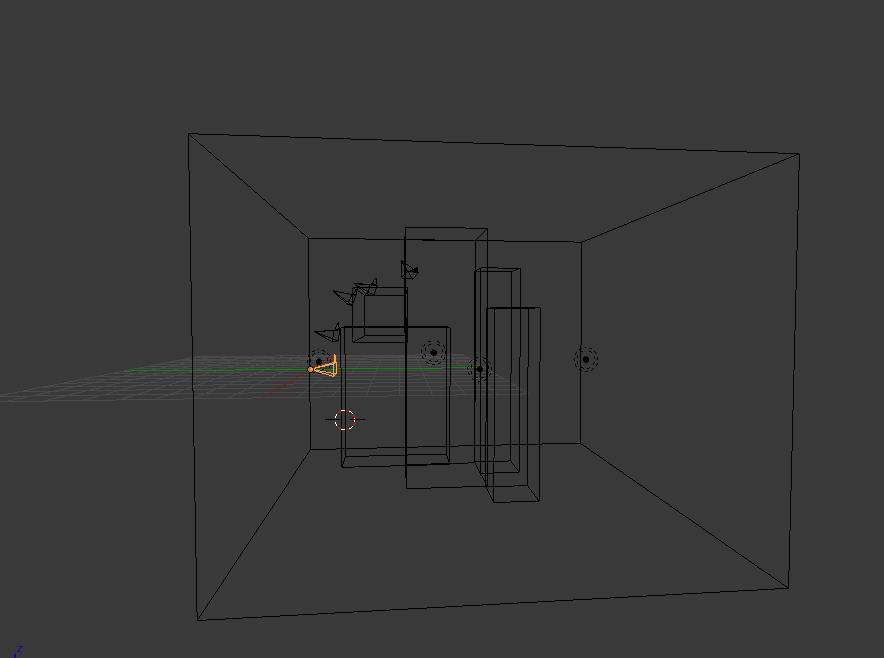
\includegraphics[width=\textwidth]{img/test6_4}
	\end{subfigure}
	%
	\begin{subfigure}{0.8\textwidth}
		\centering
		\includegraphics[width=\textwidth]{img/test6_5}
	\end{subfigure}
	%
	\caption{The first computer-generated environment we use in our test and
	an example equirectangular image from this scene.}
    \label{fig:test6}
\end{figure}
%

In the second synthetic scene we recreated a town square sourrounded by
a covered walk (loggia). The roof of the walk is sorrected by columns on the inner
side, the one that is oriented toward the square's centre, and by a wall on the
outer side.
Again the environment is contained in a room and every surface is textured.
The camera moves along the walk with a non-uniform speed while pointing toward
the centre of the square. Figure~\ref{fig:test_square} shows some images
for this second environment.
%
\begin{figure}
\centering
	\begin{subfigure}{0.4\textwidth}
		\centering
		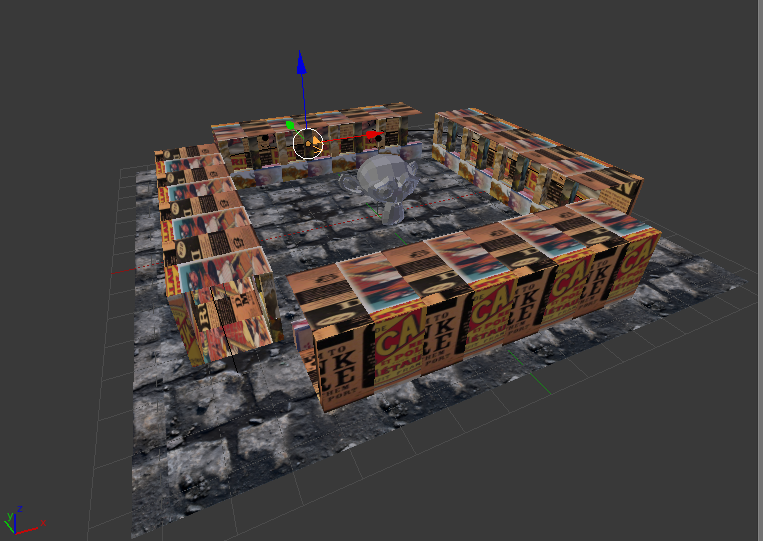
\includegraphics[width=\textwidth]{img/square1}
	\end{subfigure}
    %
	\begin{subfigure}{0.4\textwidth}
		\centering
		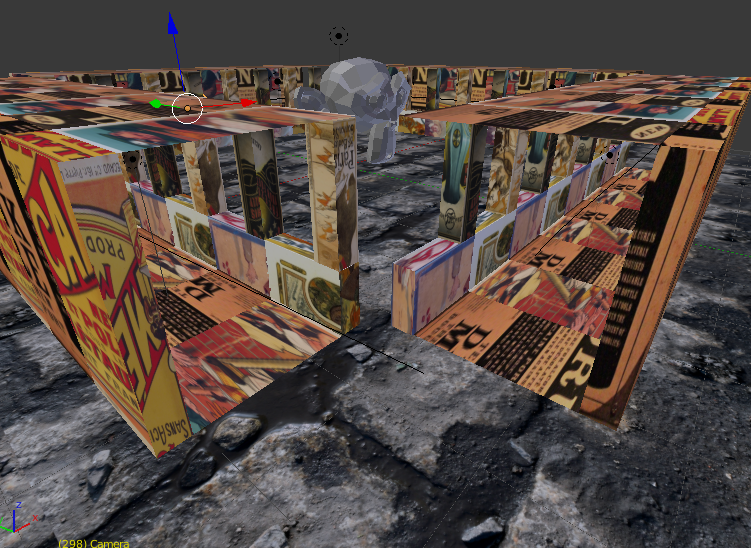
\includegraphics[width=\textwidth]{img/square2}
	\end{subfigure}
    %
	\begin{subfigure}{0.8\textwidth}
		\centering
		\includegraphics[width=\textwidth]{img/square3}
	\end{subfigure}
    %
	\begin{subfigure}{0.8\textwidth}
		\centering
		\includegraphics[width=\textwidth]{img/square4}
	\end{subfigure}
	%
	\caption{The computer-generated town square and a couple of example
	equirectangual images from this environment.}
    \label{fig:test_square}
\end{figure}

\section{Real environment}
We test our pipeline with a real video footage too. We do have the ground truth
for the camera poses in the real environment but the quality of the
reconstruction is an indicator of the pipeline performance.
We captured the real sequence with the Ricoh Theta S camera in a town square
sourrounded by a loggia. Again we walked around the square, along the covered
walks, keeping the camera above the user's head thanks to a stick.
The user do not influenced the camera poses estimation since it appears in the
pole region of the image sphere and, as we said in
Section~\ref{sec:pipeline_pose_estimation}, we discard potential matches in
these areas.
We present some pictures of the real environment toghether with some examples
of the equirectangular images of the town square in Figure~\todo{REF}.
%
\missingfigure{aggiungere foto piazza leoni}
